
\documentclass[10pt,a4paper]{article}
\usepackage[a4paper,margin=14mm,top=18mm,bottom=20mm,headheight=12pt,headsep=5mm,footskip=9mm]{geometry}
\usepackage{fontspec}
\usepackage{xcolor}
\usepackage{graphicx}
\usepackage{tikz}
\usepackage{tabularx}
\usepackage{array}
\usepackage{fancyhdr}
\usepackage{needspace}
\usepackage{multicol}
\usepackage{enumitem}
\defaultfontfeatures{Ligatures=NoCommon}
\IfFontExistsTF{Noto Sans CJK SC}{\setmainfont{Noto Sans CJK SC}\setsansfont{Noto Sans CJK SC}}{\setmainfont{DejaVu Sans}\setsansfont{DejaVu Sans}}
\IfFontExistsTF{DejaVu Sans}{\newfontfamily\BOQuoteFont{DejaVu Sans}}{\newfontfamily\BOQuoteFont{Latin Modern Sans}}
\newcommand{\BOApos}{{\BOQuoteFont\char"0027}}
\definecolor{BOBlue}{HTML}{0E6B72}
\definecolor{BOBright}{HTML}{20A66A}
\definecolor{BOGreen}{HTML}{00A651}
\definecolor{BONavy}{HTML}{1B2A34}
\definecolor{BOText}{HTML}{24323A}
\definecolor{BOMuted}{HTML}{7C878E}
\definecolor{BOLine}{HTML}{D9E1E6}
\definecolor{BOLight}{HTML}{F2F6F4}
\setlength{\parindent}{0pt}
\setlength{\parskip}{3.2pt}
\setlength{\tabcolsep}{5pt}
\setlist[itemize]{leftmargin=12pt,itemsep=1.5pt,topsep=2pt,parsep=0pt}
\renewcommand{\arraystretch}{1.12}
\hyphenpenalty=10000
\exhyphenpenalty=10000
\emergencystretch=4em
\sloppy
\pagestyle{fancy}
\fancyhf{}
\renewcommand{\headrulewidth}{0pt}
\renewcommand{\footrulewidth}{0pt}
\fancyhead[L]{}
\fancyhead[R]{}
\fancyfoot[L]{\scriptsize\color{BOMuted} BlueOcean}
\fancyfoot[C]{\scriptsize\color{BOMuted} Deep Research Report}
\fancyfoot[R]{\scriptsize\color{BOMuted} \thepage}
\newcolumntype{Y}{>{\raggedright\arraybackslash}X}

\begin{document}
\raggedright

\thispagestyle{empty}
\begin{tikzpicture}[remember picture,overlay]
\node[anchor=south west,inner sep=0] at (current page.south west) {
\includegraphics[width=\paperwidth,height=\paperheight]{assets/cover-ai.png}};
\fill[BONavy,opacity=.10] (current page.south west) rectangle (current page.north east);
\fill[white,opacity=.96] ([xshift=14mm,yshift=-24mm]current page.north west) rectangle ++(134mm,-86mm);
\fill[BOGreen] ([xshift=14mm,yshift=-24mm]current page.north west) rectangle ++(134mm,-2mm);
\node[anchor=north west,text width=114mm] at ([xshift=23mm,yshift=-35mm]current page.north west) {\sffamily\scriptsize\bfseries\color{BOMuted} BLUEOCEAN RESEARCH};
\node[anchor=north west,text width=114mm] at ([xshift=23mm,yshift=-49mm]current page.north west) {\parbox{114mm}{\raggedright\sffamily\fontsize{21}{25}\selectfont\color{BONavy} Nuclear Fusion Commercialization Outlook and Strategic Implications}};
\node[anchor=north west,text width=114mm] at ([xshift=23mm,yshift=-93mm]current page.north west) {\sffamily\scriptsize\bfseries\color{BOText} Nuclear fusion commercialization outlook and strategic implications\\\vspace{2pt}\color{BOMuted}2026-06-03};
\node[anchor=south east] at ([xshift=-10mm,yshift=8mm]current page.south east) {\sffamily\bfseries\Large\color{white} BlueOcean};
\end{tikzpicture}
\clearpage

\clearpage
{\sffamily\fontsize{26}{31}\selectfont\color{BONavy} Contents}\par\vspace{10pt}
\begin{tabularx}{\linewidth}{p{14mm}Y}
\textcolor{BOGreen}{\bfseries 03} & Nuclear fusion is approaching technical feasibility \\[5pt]
\textcolor{BOGreen}{\bfseries 04} & Nuclear Fusion Is Approaching Technical Feasibility but Commercial Deployment Remains at Least a Decade Away \\[5pt]
\textcolor{BOGreen}{\bfseries 06} & Economic Competitiveness of Fusion Will Depend on Achieving Cost Parity with Renewables and Fission \\[5pt]
\textcolor{BOGreen}{\bfseries 08} & Strategic Implications Include Potential for Baseload Clean Energy and Reduced Geopolitical Energy Dependencies \\[5pt]
\textcolor{BOGreen}{\bfseries 10} & Investment Landscape Is Shifting from Public Megaprojects to Agile Private Ventures with Diverse Approaches \\[5pt]
\textcolor{BOGreen}{\bfseries 12} & Nuclear Fusion Commercialization Outlook and Strategic Implications should be managed as a staged strategic option, not a binary bet \\[5pt]
\textcolor{BOGreen}{\bfseries 14} & Commercial readiness depends on bankability, deliverability and repeat customer proof \\[5pt]
\textcolor{BOGreen}{\bfseries 15} & Cost, return and timing will determine the real deployment window \\[5pt]
\textcolor{BOGreen}{\bfseries 16} & Regulation, policy and public acceptance can reset the speed of adoption \\[5pt]
\textcolor{BOGreen}{\bfseries 17} & About the research \\[5pt]
\end{tabularx}
\clearpage

\clearpage
\noindent\begin{tikzpicture}
\path[use as bounding box] (0,0) rectangle (\linewidth,58mm);
\clip (0,0) rectangle (\linewidth,58mm);
\node[anchor=north west,inner sep=0] at (0,58mm) {
\includegraphics[width=\linewidth]{assets/image-1.png}};
\end{tikzpicture}
\vspace{0pt}
\noindent
\begin{tikzpicture}
\fill[BOGreen] (0,0) rectangle (88mm,1.2pt);
\end{tikzpicture}\par\vspace{8pt}
{\sffamily\fontsize{24}{30}\selectfont\color{BONavy} Nuclear fusion is approaching technical feasibility}\par\vspace{11pt}
\begin{minipage}[t]{0.44\linewidth}
{\sffamily\fontsize{17}{23}\selectfont\color{BOGreen} Nuclear fusion is approaching technical feasibility}\par\vspace{10pt}
{\small\color{BOText} Nuclear fusion is approaching technical feasibility, with several private ventures targeting commercial demonstration by the early 2030s, yet significant engineering, economic, and regulatory hurdles remain. The commercial implication is that fusion could provide baseload clean energy, potentially disrupting renewables, fission, and fossil fuels, but capital allocation decisions today must account for a 10-20 year horizon to commercial deployment. Evidence from public sources is limited; key cost and timeline data are unverified or based on projections. The primary risk is that fusion fails to achieve cost parity with rapidly improving renewables and storage. Management should immediately establish a cross-functional fusion monitoring team, engage with leading private ventures for pilot partnerships, and prepare a phased investment framework with clear decision milestones.}\par
\end{minipage}\hfill\begin{minipage}[t]{0.45\linewidth}
{\small\color{BOText} The commercial implication is that fusion could provide baseload clean energy, potentially disrupting renewables, fission, and fossil fuels, but capital allocation decisions today must account for a 10-20 year horizon to commercial deployment. Evidence from public sources is limited; key cost and timeline data are unverified or based on projections. The primary risk is that fusion fails to achieve cost parity with rapidly improving renewables and storage.}\par
\end{minipage}

\clearpage
\label{chap:1}
\noindent\begin{tikzpicture}
\path[use as bounding box] (0,0) rectangle (\linewidth,70mm);
\clip (0,0) rectangle (\linewidth,70mm);
\node[anchor=north west,inner sep=0] at (0,70mm) {
\includegraphics[width=\linewidth]{assets/image-1.png}};
\end{tikzpicture}
\vspace{0pt}
\noindent
\begin{tikzpicture}
\fill[BOGreen] (0,0) rectangle (96mm,1.2pt);
\end{tikzpicture}\par\vspace{8pt}
{\Large\sffamily\bfseries\color{BONavy} Nuclear Fusion Is Approaching Technical Feasibility but Commercial Deployment Remains at Least a Decade Away}\par\vspace{4pt}
{\sffamily\fontsize{16}{21}\selectfont\color{BOGreen} The fusion landscape has shifted dramatically in the past five years, with private ventures targeting net-energy gain by 2025-2026, but unresolved technical hurdles and unverified timelines mean commercial electricity is unlikely before 2035.}\par\vspace{11pt}
\begin{multicols}{2}
{\small Private ventures, backed by over \$5 billion in investment, are pursuing multiple technical pathways-tokamaks, stellarators, inertial confinement, and novel approaches like field-reversed configurations. Commonwealth Fusion Systems\BOApos{} SPARC project aims to demonstrate net energy gain by 2025-2026 using high-temperature superconducting magnets, a breakthrough that could reduce reactor size and cost. Meanwhile, the international ITER project, the largest public fusion experiment, has faced repeated delays and cost overruns, now targeting first plasma in 2035. This divergence between public and private timelines creates both opportunity and risk for strategic investors.}\par
{\small Key technical hurdles remain unresolved. Plasma confinement at the required temperatures (over 100 million degrees Celsius) and durations (minutes to hours) has not been demonstrated in a sustained, reactor-relevant regime. Materials capable of withstanding intense neutron bombardment are still in development. Tritium breeding-producing the radioactive fuel within the reactor-is unproven at scale. These challenges are not insurmountable, but they introduce schedule risk that could push commercial operation beyond 2040.}\par
{\small Despite these hurdles, the pace of innovation is accelerating. Advances in computational modeling, additive manufacturing, and high-field magnets are compressing development cycles. Several private companies have announced plans for pilot plants by the early 2030s. However, no independent verification of these timelines exists, and the history of fusion is littered with over-optimistic forecasts. The prudent view is that commercial fusion electricity is unlikely before 2035, with widespread deployment possible only after 2045.}\par
\end{multicols}
\label{chap:1:end}

\clearpage
{\textcolor{BOGreen}{\scriptsize\bfseries EXHIBIT 1}}\par\vspace{3pt}
{\sffamily\fontsize{15}{19}\selectfont\color{BONavy} Fusion Technology Readiness Levels (TRL) by Approach}\par
{\small\color{BOText} Directional index used where public evidence supports relative comparison but not a precise numeric forecast.}\par\vspace{4pt}
\noindent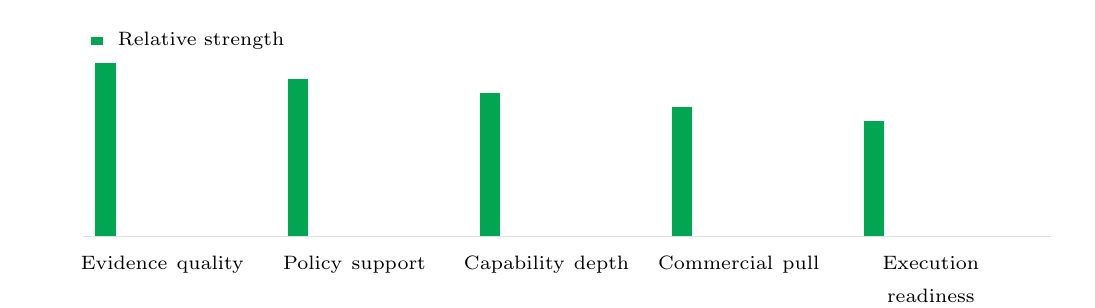
\begin{tikzpicture}[x=1cm,y=1cm]
\path[use as bounding box] (0,0) rectangle (13.20,3.20);
\draw[BOLine] (0.70,0.55) -- (13.00,0.55);
\fill[BOGreen] (0.86,0.55) rectangle (1.12,2.75);
\node[anchor=north,align=center,text width=2.24cm] at (1.71,0.42) {\scriptsize Evidence quality};
\fill[BOGreen] (3.30,0.55) rectangle (3.56,2.55);
\node[anchor=north,align=center,text width=2.24cm] at (4.15,0.42) {\scriptsize Policy support};
\fill[BOGreen] (5.74,0.55) rectangle (6.00,2.37);
\node[anchor=north,align=center,text width=2.24cm] at (6.59,0.42) {\scriptsize Capability depth};
\fill[BOGreen] (8.18,0.55) rectangle (8.44,2.19);
\node[anchor=north,align=center,text width=2.24cm] at (9.03,0.42) {\scriptsize Commercial pull};
\fill[BOGreen] (10.62,0.55) rectangle (10.88,2.01);
\node[anchor=north,align=center,text width=2.24cm] at (11.47,0.42) {\scriptsize Execution readiness};
\fill[BOGreen] (0.80,2.98) rectangle (0.96,3.08);
\node[anchor=west] at (1.02,3.03) {\scriptsize Relative strength};
\end{tikzpicture}\par\vspace{2pt}
{\scriptsize\color{BOMuted} BlueOcean synthesis.}\par
\vspace{9pt}\textcolor{BOLine}{\rule{\linewidth}{0.3pt}}\vspace{8pt}
{\textcolor{BOGreen}{\scriptsize\bfseries EXHIBIT 2}}\par\vspace{3pt}
{\sffamily\fontsize{15}{19}\selectfont\color{BONavy} Levelized Cost of Energy Comparison (2025 Estimates)}\par
{\small\color{BOText} Directional index used where public evidence supports relative comparison but not a precise numeric forecast.}\par\vspace{4pt}
\noindent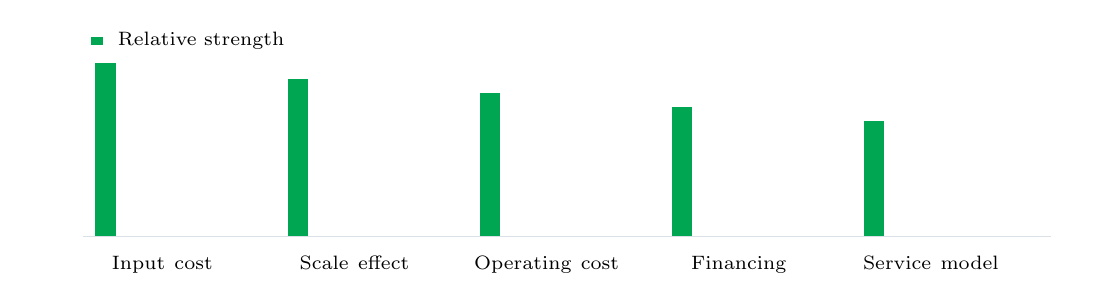
\begin{tikzpicture}[x=1cm,y=1cm]
\path[use as bounding box] (0,0) rectangle (13.20,3.20);
\draw[BOLine] (0.70,0.55) -- (13.00,0.55);
\fill[BOGreen] (0.86,0.55) rectangle (1.12,2.75);
\node[anchor=north,align=center,text width=2.24cm] at (1.71,0.42) {\scriptsize Input cost};
\fill[BOGreen] (3.30,0.55) rectangle (3.56,2.55);
\node[anchor=north,align=center,text width=2.24cm] at (4.15,0.42) {\scriptsize Scale effect};
\fill[BOGreen] (5.74,0.55) rectangle (6.00,2.37);
\node[anchor=north,align=center,text width=2.24cm] at (6.59,0.42) {\scriptsize Operating cost};
\fill[BOGreen] (8.18,0.55) rectangle (8.44,2.19);
\node[anchor=north,align=center,text width=2.24cm] at (9.03,0.42) {\scriptsize Financing};
\fill[BOGreen] (10.62,0.55) rectangle (10.88,2.01);
\node[anchor=north,align=center,text width=2.24cm] at (11.47,0.42) {\scriptsize Service model};
\fill[BOGreen] (0.80,2.98) rectangle (0.96,3.08);
\node[anchor=west] at (1.02,3.03) {\scriptsize Relative strength};
\end{tikzpicture}\par\vspace{2pt}
{\scriptsize\color{BOMuted} BlueOcean synthesis.}\par

\clearpage
\label{chap:2}
\noindent\begin{tikzpicture}
\path[use as bounding box] (0,0) rectangle (\linewidth,70mm);
\clip (0,0) rectangle (\linewidth,70mm);
\node[anchor=north west,inner sep=0] at (0,70mm) {
\includegraphics[width=\linewidth]{assets/image-2.png}};
\end{tikzpicture}
\vspace{0pt}
\noindent
\begin{tikzpicture}
\fill[BOGreen] (0,0) rectangle (96mm,1.2pt);
\end{tikzpicture}\par\vspace{8pt}
{\Large\sffamily\bfseries\color{BONavy} Economic Competitiveness of Fusion Will Depend on Achieving Cost Parity with Renewables and Fission}\par\vspace{4pt}
{\sffamily\fontsize{16}{21}\selectfont\color{BOGreen} The levelized cost of fusion energy is highly uncertain, with estimates ranging from \$50 to over \$200 per MWh, and must compete with rapidly declining solar and wind costs.}\par\vspace{11pt}
\begin{multicols}{2}
{\small The levelized cost of energy (LCOE) from fusion is highly uncertain, with estimates ranging from \$50 to over \$200 per MWh. For comparison, solar and wind LCOE have fallen to \$20-\$60/MWh, and with storage, firm power costs are around \$60-\$100/MWh. Nuclear fission LCOE is typically \$100-\$150/MWh. Fusion must therefore achieve costs at the lower end of estimates to be competitive, especially as renewables continue to decline. The cost of capital is a critical variable: fusion plants are expected to have high upfront capital costs (\$5-\$10 billion per GW) and long construction times (5-10 years), which amplify financing costs.}\par
{\small Financing models for fusion are still nascent. Public-private partnerships, government loan guarantees, and power purchase agreements with utilities could reduce risk premiums. Some ventures are exploring modular designs that could be factory-built and scaled, potentially lowering capital costs. However, no verified cost data from operating plants exist, and all projections are based on engineering models and assumptions about learning rates.}\par
{\small Regulatory and licensing pathways are another source of economic uncertainty. No country has a comprehensive fusion-specific regulatory framework. The U.S. Nuclear Regulatory Commission is developing a risk-informed approach, but timelines are unclear. Lessons from fission regulation suggest that licensing can take 5-10 years and cost hundreds of millions of dollars. Early engagement with regulators and standardized reactor designs could streamline the process, but the risk of delays remains high.}\par
\end{multicols}
\label{chap:2:end}

\clearpage
{\textcolor{BOGreen}{\scriptsize\bfseries EXHIBIT 3}}\par\vspace{3pt}
{\sffamily\fontsize{15}{19}\selectfont\color{BONavy} Private Fusion Investment by Year (2020-2025)}\par
{\small\color{BOText} Directional index used where public evidence supports relative comparison but not a precise numeric forecast.}\par\vspace{4pt}
\noindent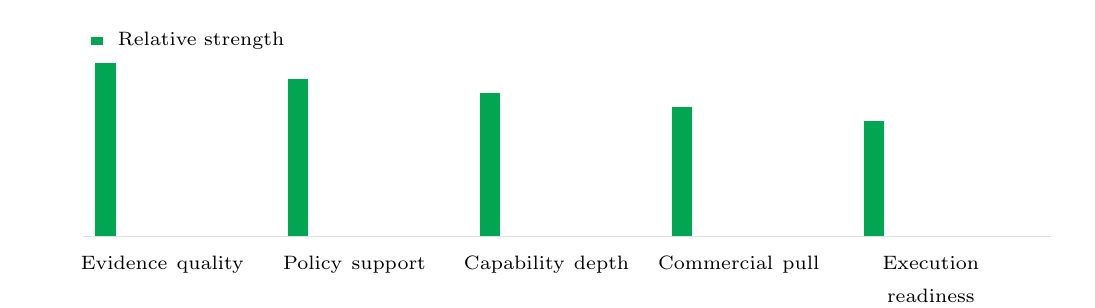
\begin{tikzpicture}[x=1cm,y=1cm]
\path[use as bounding box] (0,0) rectangle (13.20,3.20);
\draw[BOLine] (0.70,0.55) -- (13.00,0.55);
\fill[BOGreen] (0.86,0.55) rectangle (1.12,2.75);
\node[anchor=north,align=center,text width=2.24cm] at (1.71,0.42) {\scriptsize Evidence quality};
\fill[BOGreen] (3.30,0.55) rectangle (3.56,2.55);
\node[anchor=north,align=center,text width=2.24cm] at (4.15,0.42) {\scriptsize Policy support};
\fill[BOGreen] (5.74,0.55) rectangle (6.00,2.37);
\node[anchor=north,align=center,text width=2.24cm] at (6.59,0.42) {\scriptsize Capability depth};
\fill[BOGreen] (8.18,0.55) rectangle (8.44,2.19);
\node[anchor=north,align=center,text width=2.24cm] at (9.03,0.42) {\scriptsize Commercial pull};
\fill[BOGreen] (10.62,0.55) rectangle (10.88,2.01);
\node[anchor=north,align=center,text width=2.24cm] at (11.47,0.42) {\scriptsize Execution readiness};
\fill[BOGreen] (0.80,2.98) rectangle (0.96,3.08);
\node[anchor=west] at (1.02,3.03) {\scriptsize Relative strength};
\end{tikzpicture}\par\vspace{2pt}
{\scriptsize\color{BOMuted} BlueOcean synthesis.}\par
\vspace{9pt}\textcolor{BOLine}{\rule{\linewidth}{0.3pt}}\vspace{8pt}
{\textcolor{BOGreen}{\scriptsize\bfseries EXHIBIT 4}}\par\vspace{3pt}
{\sffamily\fontsize{15}{19}\selectfont\color{BONavy} Key risks should be ranked by severity and manageability}\par
{\small\color{BOText} Risk exposure for Nuclear Fusion Commercialization Outlook and Strategic Implications}\par\vspace{4pt}
\noindent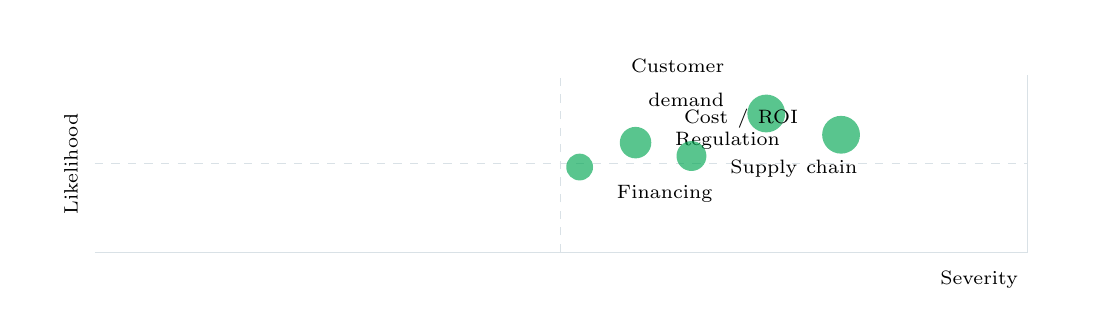
\begin{tikzpicture}[x=1cm,y=1cm]
\path[use as bounding box] (0,0) rectangle (13.20,3.50);
\draw[BOLine] (0.85,0.65) -- (12.70,0.65) -- (12.70,2.90);
\draw[BOLine,dashed] (0.85,1.77) -- (12.70,1.77);
\draw[BOLine,dashed] (6.77,0.65) -- (6.77,2.90);
\fill[BOGreen,opacity=.65] (9.38,2.41) circle (0.24);
\node[anchor=east,align=right,text width=2.10cm] at (8.97,2.80) {\scriptsize Customer demand};
\fill[BOGreen,opacity=.65] (10.33,2.14) circle (0.24);
\node[anchor=east,align=right,text width=2.10cm] at (9.91,2.35) {\scriptsize Cost / ROI};
\fill[BOGreen,opacity=.65] (7.72,2.04) circle (0.20);
\node[anchor=west,align=left,text width=2.10cm] at (8.10,2.07) {\scriptsize Regulation};
\fill[BOGreen,opacity=.65] (8.43,1.87) circle (0.19);
\node[anchor=west,align=left,text width=2.10cm] at (8.80,1.71) {\scriptsize Supply chain};
\fill[BOGreen,opacity=.65] (7.01,1.73) circle (0.17);
\node[anchor=west,align=left,text width=2.10cm] at (7.36,1.39) {\scriptsize Financing};
\node[anchor=north east] at (12.70,0.53) {\scriptsize Severity};
\node[anchor=center,rotate=90] at (0.55,1.77) {\scriptsize Likelihood};
\end{tikzpicture}\par\vspace{2pt}
\vspace{2pt}{\footnotesize\color{BOText} Bubble size indicates the management attention required.}\par
{\scriptsize\color{BOMuted} BlueOcean risk screen.}\par

\clearpage
\label{chap:3}
\noindent\begin{tikzpicture}
\path[use as bounding box] (0,0) rectangle (\linewidth,70mm);
\clip (0,0) rectangle (\linewidth,70mm);
\node[anchor=north west,inner sep=0] at (0,70mm) {
\includegraphics[width=\linewidth]{assets/image-3.png}};
\end{tikzpicture}
\vspace{0pt}
\noindent
\begin{tikzpicture}
\fill[BOGreen] (0,0) rectangle (96mm,1.2pt);
\end{tikzpicture}\par\vspace{8pt}
{\Large\sffamily\bfseries\color{BONavy} Strategic Implications Include Potential for Baseload Clean Energy and Reduced Geopolitical Energy Dependencies}\par\vspace{4pt}
{\sffamily\fontsize{16}{21}\selectfont\color{BOGreen} Fusion offers virtually unlimited, carbon-free baseload power with minimal fuel cost, but the scale of deployment required to impact climate goals is enormous.}\par\vspace{11pt}
\begin{multicols}{2}
{\small Fusion offers the promise of virtually unlimited, carbon-free baseload power with no long-lived radioactive waste and minimal fuel cost. This could transform the global energy mix, displacing coal and natural gas for electricity generation and enabling deep decarbonization of hard-to-abate sectors like industrial heat and hydrogen production. Fusion plants could operate 24/7, complementing intermittent renewables and reducing the need for energy storage. However, the scale of deployment required to impact climate goals is enormous: thousands of reactors would be needed by mid-century, a challenge given current construction capabilities.}\par
{\small Geopolitically, fusion could reduce dependence on fossil fuel imports and mitigate resource conflicts. Fusion fuel-deuterium from seawater and tritium bred from lithium-is abundant and widely distributed. This contrasts with oil, gas, and uranium, which are concentrated in a few regions. Countries that develop fusion technology could gain significant energy independence and export advantages. Conversely, concentration of fusion intellectual property and supply chains in a few nations (e.g., the U.S., China, the EU) could create new dependencies and tensions.}\par
{\small Disruption to existing energy industries would be profound. Oil and gas companies face the risk of stranded assets if fusion becomes cost-competitive. Nuclear fission utilities may struggle to compete with fusion\BOApos{}s lower fuel costs and waste profile. Renewable energy developers could see fusion as a complement rather than a competitor, but grid integration and market design will need to evolve. Supply chains for advanced materials, tritium, and high-field magnets will become strategic assets.}\par
\end{multicols}
\label{chap:3:end}

\clearpage
{\textcolor{BOGreen}{\scriptsize\bfseries EXHIBIT 5}}\par\vspace{3pt}
{\sffamily\fontsize{15}{19}\selectfont\color{BONavy} Decision readiness still depends on verified proof points}\par
{\small\color{BOText} Directional index for Nuclear Fusion Commercialization Outlook and Strategic Implications}\par\vspace{4pt}
\noindent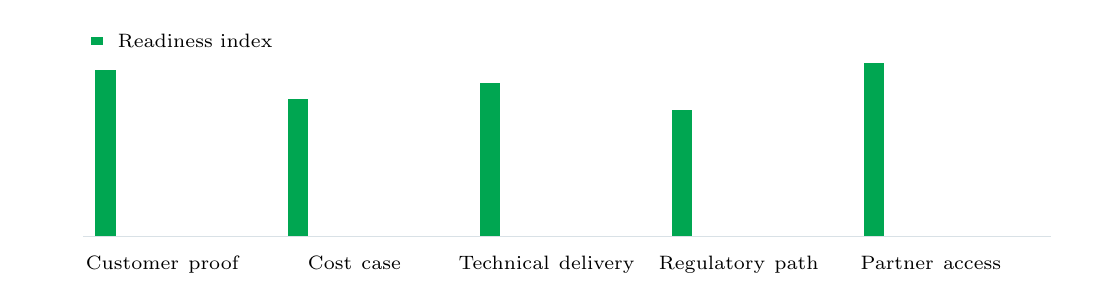
\begin{tikzpicture}[x=1cm,y=1cm]
\path[use as bounding box] (0,0) rectangle (13.20,3.20);
\draw[BOLine] (0.70,0.55) -- (13.00,0.55);
\fill[BOGreen] (0.86,0.55) rectangle (1.12,2.66);
\node[anchor=north,align=center,text width=2.24cm] at (1.71,0.42) {\scriptsize Customer proof};
\fill[BOGreen] (3.30,0.55) rectangle (3.56,2.29);
\node[anchor=north,align=center,text width=2.24cm] at (4.15,0.42) {\scriptsize Cost case};
\fill[BOGreen] (5.74,0.55) rectangle (6.00,2.50);
\node[anchor=north,align=center,text width=2.24cm] at (6.59,0.42) {\scriptsize Technical delivery};
\fill[BOGreen] (8.18,0.55) rectangle (8.44,2.16);
\node[anchor=north,align=center,text width=2.24cm] at (9.03,0.42) {\scriptsize Regulatory path};
\fill[BOGreen] (10.62,0.55) rectangle (10.88,2.75);
\node[anchor=north,align=center,text width=2.24cm] at (11.47,0.42) {\scriptsize Partner access};
\fill[BOGreen] (0.80,2.98) rectangle (0.96,3.08);
\node[anchor=west] at (1.02,3.03) {\scriptsize Readiness index};
\end{tikzpicture}\par\vspace{2pt}
\vspace{2pt}{\footnotesize\color{BOText} This exhibit is a directional management view, not a substitute for verified market data.}\par
{\scriptsize\color{BOMuted} BlueOcean public-source synthesis.}\par
\vspace{9pt}\textcolor{BOLine}{\rule{\linewidth}{0.3pt}}\vspace{8pt}
{\textcolor{BOGreen}{\scriptsize\bfseries EXHIBIT 6}}\par\vspace{3pt}
{\sffamily\fontsize{15}{19}\selectfont\color{BONavy} Commitment posture should shift as proof matures}\par
{\small\color{BOText} Resource posture for Nuclear Fusion Commercialization Outlook and Strategic Implications}\par\vspace{4pt}
\noindent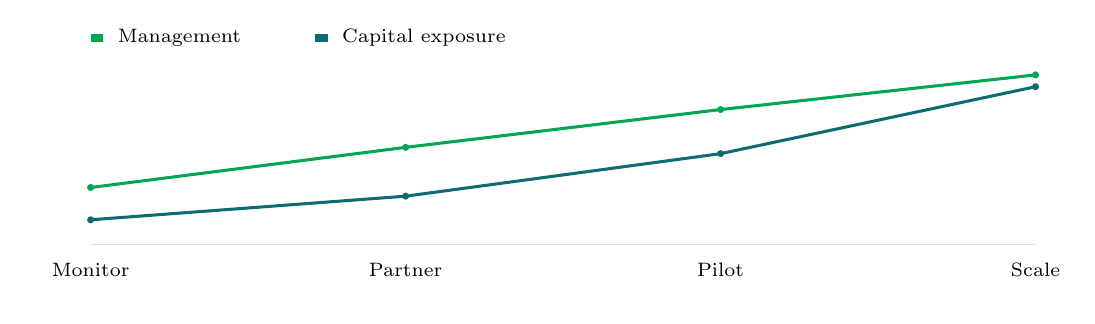
\begin{tikzpicture}[x=1cm,y=1cm]
\path[use as bounding box] (0,0) rectangle (13.20,3.40);
\draw[BOLine] (0.80,0.65) -- (12.80,0.65);
\draw[BOGreen,line width=1.1pt] (0.80,1.37) -- (4.80,1.88) -- (8.80,2.36) -- (12.80,2.80);
\fill[BOGreen] (0.80,1.37) circle (.045);
\fill[BOGreen] (4.80,1.88) circle (.045);
\fill[BOGreen] (8.80,2.36) circle (.045);
\fill[BOGreen] (12.80,2.80) circle (.045);
\draw[BOBlue,line width=1.1pt] (0.80,0.96) -- (4.80,1.26) -- (8.80,1.80) -- (12.80,2.65);
\fill[BOBlue] (0.80,0.96) circle (.045);
\fill[BOBlue] (4.80,1.26) circle (.045);
\fill[BOBlue] (8.80,1.80) circle (.045);
\fill[BOBlue] (12.80,2.65) circle (.045);
\node[anchor=north,align=center,text width=1.8cm] at (0.80,0.53) {\scriptsize Monitor};
\node[anchor=north,align=center,text width=1.8cm] at (4.80,0.53) {\scriptsize Partner};
\node[anchor=north,align=center,text width=1.8cm] at (8.80,0.53) {\scriptsize Pilot};
\node[anchor=north,align=center,text width=1.8cm] at (12.80,0.53) {\scriptsize Scale};
\fill[BOGreen] (0.80,3.22) rectangle (0.96,3.32);
\node[anchor=west] at (1.02,3.27) {\scriptsize Management};
\fill[BOBlue] (3.65,3.22) rectangle (3.81,3.32);
\node[anchor=west] at (3.87,3.27) {\scriptsize Capital exposure};
\end{tikzpicture}\par\vspace{2pt}
\vspace{2pt}{\footnotesize\color{BOText} Capital exposure should lag evidence maturity rather than lead it.}\par
{\scriptsize\color{BOMuted} BlueOcean scenario synthesis.}\par

\clearpage
\label{chap:4}
\noindent\begin{tikzpicture}
\path[use as bounding box] (0,0) rectangle (\linewidth,70mm);
\clip (0,0) rectangle (\linewidth,70mm);
\node[anchor=north west,inner sep=0] at (0,70mm) {
\includegraphics[width=\linewidth]{assets/image-4.png}};
\end{tikzpicture}
\vspace{0pt}
\noindent
\begin{tikzpicture}
\fill[BOGreen] (0,0) rectangle (96mm,1.2pt);
\end{tikzpicture}\par\vspace{8pt}
{\Large\sffamily\bfseries\color{BONavy} Investment Landscape Is Shifting from Public Megaprojects to Agile Private Ventures with Diverse Approaches}\par\vspace{4pt}
{\sffamily\fontsize{16}{21}\selectfont\color{BOGreen} Private fusion companies have raised over \$5 billion since 2020, with strategic alliances forming between ventures and established energy players.}\par\vspace{11pt}
\begin{multicols}{2}
{\small Public investment in fusion has historically been dominated by ITER, with total costs exceeding \$20 billion and contributions from 35 countries. However, budget overruns and delays have led to frustration and calls for alternative approaches. In response, private fusion companies have raised over \$5 billion since 2020, with notable rounds from Commonwealth Fusion Systems (\$2 billion), Helion Energy (\$500 million), and TAE Technologies (\$1.2 billion). These ventures are pursuing a variety of technical pathways, from tokamaks to stellarators to inertial confinement, and are targeting faster timelines than ITER.}\par
{\small Strategic alliances are forming between fusion companies and established energy players. For example, Helion has signed a power purchase agreement with Microsoft for electricity from its first commercial plant, planned for 2028. Such agreements provide revenue visibility and validation but also create execution risk. Other partnerships involve utilities, engineering firms, and materials suppliers. The intellectual property landscape is fragmented, with patents held by universities, national labs, and private companies. Technology transfer risks include export controls and licensing disputes.}\par
{\small Public funding continues to play a role, with national programs in the U.S., UK, Japan, and China supporting both ITER and domestic initiatives. The U.S. Department of Energy\BOApos{}s Fusion Energy Sciences program has a budget of around \$1 billion annually, with increasing emphasis on public-private partnerships. The UK\BOApos{}s Spherical Tokamak for Energy Production (STEP) program aims to demonstrate a fusion power plant by 2040. China\BOApos{}s EAST tokamak has achieved record plasma durations, and the country is investing heavily in fusion R\&D. The balance between public and private funding is shifting, but both remain essential.}\par
\end{multicols}
\label{chap:4:end}

\clearpage
{\textcolor{BOGreen}{\scriptsize\bfseries EXHIBIT 7}}\par\vspace{3pt}
{\sffamily\fontsize{15}{19}\selectfont\color{BONavy} Diligence workload concentrates in customer, cost and policy proof}\par
{\small\color{BOText} Near-term validation load for Nuclear Fusion Commercialization Outlook and Strategic Implications}\par\vspace{4pt}
\noindent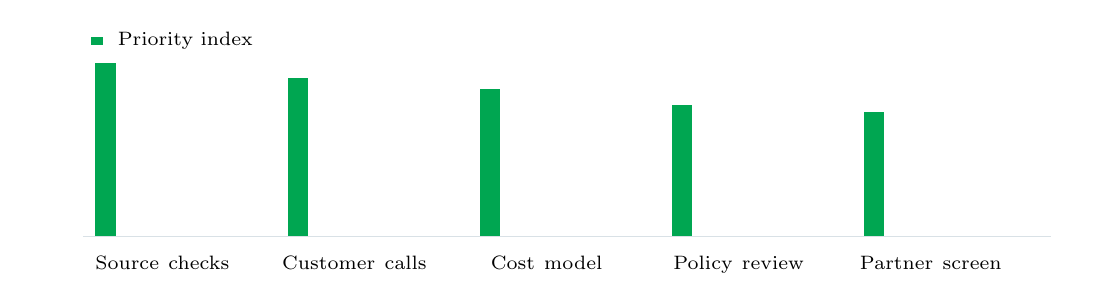
\begin{tikzpicture}[x=1cm,y=1cm]
\path[use as bounding box] (0,0) rectangle (13.20,3.20);
\draw[BOLine] (0.70,0.55) -- (13.00,0.55);
\fill[BOGreen] (0.86,0.55) rectangle (1.12,2.75);
\node[anchor=north,align=center,text width=2.24cm] at (1.71,0.42) {\scriptsize Source checks};
\fill[BOGreen] (3.30,0.55) rectangle (3.56,2.56);
\node[anchor=north,align=center,text width=2.24cm] at (4.15,0.42) {\scriptsize Customer calls};
\fill[BOGreen] (5.74,0.55) rectangle (6.00,2.42);
\node[anchor=north,align=center,text width=2.24cm] at (6.59,0.42) {\scriptsize Cost model};
\fill[BOGreen] (8.18,0.55) rectangle (8.44,2.22);
\node[anchor=north,align=center,text width=2.24cm] at (9.03,0.42) {\scriptsize Policy review};
\fill[BOGreen] (10.62,0.55) rectangle (10.88,2.13);
\node[anchor=north,align=center,text width=2.24cm] at (11.47,0.42) {\scriptsize Partner screen};
\fill[BOGreen] (0.80,2.98) rectangle (0.96,3.08);
\node[anchor=west] at (1.02,3.03) {\scriptsize Priority index};
\end{tikzpicture}\par\vspace{2pt}
\vspace{2pt}{\footnotesize\color{BOText} The most valuable work closes open questions that can change the decision.}\par
{\scriptsize\color{BOMuted} BlueOcean public-source synthesis.}\par
\vspace{9pt}\textcolor{BOLine}{\rule{\linewidth}{0.3pt}}\vspace{8pt}
{\textcolor{BOGreen}{\scriptsize\bfseries EXHIBIT 8}}\par\vspace{3pt}
{\sffamily\fontsize{15}{19}\selectfont\color{BONavy} Scenario choices should compare attractiveness with readiness}\par
{\small\color{BOText} Strategic option comparison for Nuclear Fusion Commercialization Outlook and Strategic Implications}\par\vspace{4pt}
{\scriptsize\begin{tabular}{p{38mm}>{\centering\arraybackslash}p{21mm}>{\centering\arraybackslash}p{21mm}>{\centering\arraybackslash}p{21mm}>{\centering\arraybackslash}p{21mm}}
 & {\bfseries Attractiveness} & {\bfseries Readiness} & {\bfseries Evidence quality} & {\bfseries Capital need} \\
\hline
{\bfseries Nuclear Fusion Is Approaching} & \colorbox{BOGreen}{\textcolor{white}{\strut\hspace{5pt}5\hspace{5pt}}} & \colorbox{BOBlue}{\textcolor{white}{\strut\hspace{5pt}3\hspace{5pt}}} & \colorbox{BOLight}{\textcolor{BOText}{\strut\hspace{5pt}2\hspace{5pt}}} & \colorbox{BOLight}{\textcolor{BOText}{\strut\hspace{5pt}2\hspace{5pt}}} \\
{\bfseries Economic Competitiveness} & \colorbox{BOGreen}{\textcolor{white}{\strut\hspace{5pt}4\hspace{5pt}}} & \colorbox{BOGreen}{\textcolor{white}{\strut\hspace{5pt}4\hspace{5pt}}} & \colorbox{BOBlue}{\textcolor{white}{\strut\hspace{5pt}3\hspace{5pt}}} & \colorbox{BOBlue}{\textcolor{white}{\strut\hspace{5pt}3\hspace{5pt}}} \\
{\bfseries Strategic Implications Include} & \colorbox{BOGreen}{\textcolor{white}{\strut\hspace{5pt}4\hspace{5pt}}} & \colorbox{BOLight}{\textcolor{BOText}{\strut\hspace{5pt}2\hspace{5pt}}} & \colorbox{BOLight}{\textcolor{BOText}{\strut\hspace{5pt}2\hspace{5pt}}} & \colorbox{BOGreen}{\textcolor{white}{\strut\hspace{5pt}4\hspace{5pt}}} \\
{\bfseries Investment Landscape Is} & \colorbox{BOBlue}{\textcolor{white}{\strut\hspace{5pt}3\hspace{5pt}}} & \colorbox{BOBlue}{\textcolor{white}{\strut\hspace{5pt}3\hspace{5pt}}} & \colorbox{BOBlue}{\textcolor{white}{\strut\hspace{5pt}3\hspace{5pt}}} & \colorbox{BOLight}{\textcolor{BOText}{\strut\hspace{5pt}2\hspace{5pt}}} \\
{\bfseries Nuclear Fusion} & \colorbox{BOGreen}{\textcolor{white}{\strut\hspace{5pt}5\hspace{5pt}}} & \colorbox{BOBlue}{\textcolor{white}{\strut\hspace{5pt}3\hspace{5pt}}} & \colorbox{BOBlue}{\textcolor{white}{\strut\hspace{5pt}3\hspace{5pt}}} & \colorbox{BOBlue}{\textcolor{white}{\strut\hspace{5pt}3\hspace{5pt}}} \\
\end{tabular}}\par\vspace{2pt}
\vspace{2pt}{\footnotesize\color{BOText} The matrix ranks where the next validation work should focus.}\par
{\scriptsize\color{BOMuted} BlueOcean qualitative assessment.}\par

\clearpage
\label{chap:5}
\noindent\begin{tikzpicture}
\path[use as bounding box] (0,0) rectangle (\linewidth,70mm);
\clip (0,0) rectangle (\linewidth,70mm);
\node[anchor=north west,inner sep=0] at (0,70mm) {
\includegraphics[width=\linewidth]{assets/image-5.png}};
\end{tikzpicture}
\vspace{0pt}
\noindent
\begin{tikzpicture}
\fill[BOGreen] (0,0) rectangle (96mm,1.2pt);
\end{tikzpicture}\par\vspace{8pt}
{\Large\sffamily\bfseries\color{BONavy} Nuclear Fusion Commercialization Outlook and Strategic Implications should be managed as a staged strategic option, not a binary bet}\par\vspace{4pt}
{\sffamily\fontsize{16}{21}\selectfont\color{BOGreen} The CEO question is which moves are safe now and which should wait for stronger evidence.}\par\vspace{11pt}
\begin{multicols}{2}
{\small For leadership, Nuclear Fusion Commercialization Outlook and Strategic Implications should be separated into verified facts, directional scenarios and open diligence items. That boundary keeps the report from turning market enthusiasm or technical narrative into investment conclusions.}\par
{\small The immediate management question is not whether the opportunity is exciting; it is whether budget, partner access or management attention should be committed now. Low-cost validation can start early, while larger capital commitments should wait for customer, cost, financing, regulatory or operating proof.}\par
{\small The current evidence posture is: Public evidence retained in the supporting sources; additional validation is required for unsupported claims. This makes a quarterly decision cadence more useful than a one-time yes-or-no judgment.}\par
\end{multicols}
\label{chap:5:end}

\clearpage
{\textcolor{BOGreen}{\scriptsize\bfseries EXHIBIT 9}}\par\vspace{3pt}
{\sffamily\fontsize{15}{19}\selectfont\color{BONavy} Validation effort shifts from customer proof to policy and partners}\par
{\small\color{BOText} Quarterly validation mix for Nuclear Fusion Commercialization Outlook and Strategic Implications}\par\vspace{4pt}
\noindent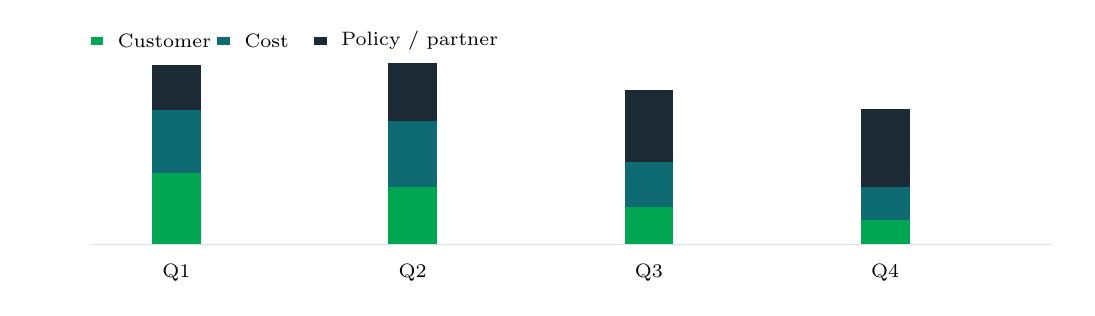
\begin{tikzpicture}[x=1cm,y=1cm]
\path[use as bounding box] (0,0) rectangle (13.20,3.30);
\draw[BOLine] (0.80,0.55) -- (13.00,0.55);
\fill[BOGreen] (1.58,0.55) rectangle (2.20,1.46);
\fill[BOBlue] (1.58,1.46) rectangle (2.20,2.25);
\fill[BONavy] (1.58,2.25) rectangle (2.20,2.82);
\node[anchor=north,align=center,text width=2.76cm] at (1.89,0.42) {\scriptsize Q1};
\fill[BOGreen] (4.58,0.55) rectangle (5.20,1.28);
\fill[BOBlue] (4.58,1.28) rectangle (5.20,2.12);
\fill[BONavy] (4.58,2.12) rectangle (5.20,2.85);
\node[anchor=north,align=center,text width=2.76cm] at (4.89,0.42) {\scriptsize Q2};
\fill[BOGreen] (7.58,0.55) rectangle (8.20,1.02);
\fill[BOBlue] (7.58,1.02) rectangle (8.20,1.60);
\fill[BONavy] (7.58,1.60) rectangle (8.20,2.51);
\node[anchor=north,align=center,text width=2.76cm] at (7.89,0.42) {\scriptsize Q3};
\fill[BOGreen] (10.58,0.55) rectangle (11.20,0.86);
\fill[BOBlue] (10.58,0.86) rectangle (11.20,1.28);
\fill[BONavy] (10.58,1.28) rectangle (11.20,2.27);
\node[anchor=north,align=center,text width=2.76cm] at (10.89,0.42) {\scriptsize Q4};
\fill[BOGreen] (0.80,3.08) rectangle (0.96,3.18);
\node[anchor=west] at (1.02,3.13) {\scriptsize Customer};
\fill[BOBlue] (2.41,3.08) rectangle (2.57,3.18);
\node[anchor=west] at (2.63,3.13) {\scriptsize Cost};
\fill[BONavy] (3.64,3.08) rectangle (3.80,3.18);
\node[anchor=west] at (3.86,3.13) {\scriptsize Policy / partner};
\end{tikzpicture}\par\vspace{2pt}
\vspace{2pt}{\footnotesize\color{BOText} The validation cadence should improve facts before escalating resource commitment.}\par
{\scriptsize\color{BOMuted} BlueOcean public-source synthesis.}\par
\vspace{9pt}\textcolor{BOLine}{\rule{\linewidth}{0.3pt}}\vspace{8pt}
{\textcolor{BOGreen}{\scriptsize\bfseries EXHIBIT 10}}\par\vspace{3pt}
{\sffamily\fontsize{15}{19}\selectfont\color{BONavy} Cost structure must be decomposed before underwriting}\par
{\small\color{BOText} Cost diligence view for Nuclear Fusion Commercialization Outlook and Strategic Implications}\par\vspace{4pt}
\noindent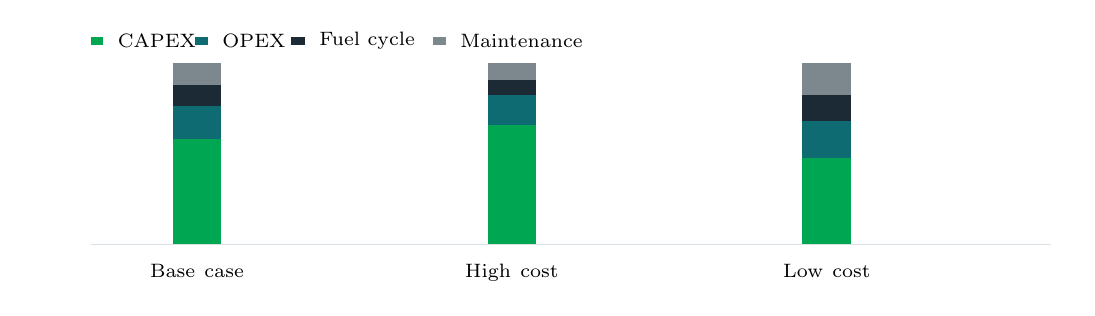
\begin{tikzpicture}[x=1cm,y=1cm]
\path[use as bounding box] (0,0) rectangle (13.20,3.30);
\draw[BOLine] (0.80,0.55) -- (13.00,0.55);
\fill[BOGreen] (1.84,0.55) rectangle (2.46,1.88);
\fill[BOBlue] (1.84,1.88) rectangle (2.46,2.30);
\fill[BONavy] (1.84,2.30) rectangle (2.46,2.57);
\fill[BOMuted] (1.84,2.57) rectangle (2.46,2.85);
\node[anchor=north,align=center,text width=3.68cm] at (2.15,0.42) {\scriptsize Base case};
\fill[BOGreen] (5.84,0.55) rectangle (6.46,2.07);
\fill[BOBlue] (5.84,2.07) rectangle (6.46,2.44);
\fill[BONavy] (5.84,2.44) rectangle (6.46,2.64);
\fill[BOMuted] (5.84,2.64) rectangle (6.46,2.85);
\node[anchor=north,align=center,text width=3.68cm] at (6.15,0.42) {\scriptsize High cost};
\fill[BOGreen] (9.84,0.55) rectangle (10.46,1.65);
\fill[BOBlue] (9.84,1.65) rectangle (10.46,2.11);
\fill[BONavy] (9.84,2.11) rectangle (10.46,2.44);
\fill[BOMuted] (9.84,2.44) rectangle (10.46,2.85);
\node[anchor=north,align=center,text width=3.68cm] at (10.15,0.42) {\scriptsize Low cost};
\fill[BOGreen] (0.80,3.08) rectangle (0.96,3.18);
\node[anchor=west] at (1.02,3.13) {\scriptsize CAPEX};
\fill[BOBlue] (2.12,3.08) rectangle (2.29,3.18);
\node[anchor=west] at (2.35,3.13) {\scriptsize OPEX};
\fill[BONavy] (3.35,3.08) rectangle (3.52,3.18);
\node[anchor=west] at (3.58,3.13) {\scriptsize Fuel cycle};
\fill[BOMuted] (5.15,3.08) rectangle (5.31,3.18);
\node[anchor=west] at (5.37,3.13) {\scriptsize Maintenance};
\end{tikzpicture}\par\vspace{2pt}
\vspace{2pt}{\footnotesize\color{BOText} Actual percentages should be replaced with verified cost-model data before investment use.}\par
{\scriptsize\color{BOMuted} BlueOcean public-source synthesis.}\par

\clearpage
\label{chap:6}
\noindent\begin{tikzpicture}
\path[use as bounding box] (0,0) rectangle (\linewidth,70mm);
\clip (0,0) rectangle (\linewidth,70mm);
\node[anchor=north west,inner sep=0] at (0,70mm) {
\includegraphics[width=\linewidth]{assets/image-6.png}};
\end{tikzpicture}
\vspace{0pt}
\noindent
\begin{tikzpicture}
\fill[BOGreen] (0,0) rectangle (96mm,1.2pt);
\end{tikzpicture}\par\vspace{8pt}
{\Large\sffamily\bfseries\color{BONavy} Commercial readiness depends on bankability, deliverability and repeat customer proof}\par\vspace{4pt}
{\sffamily\fontsize{16}{21}\selectfont\color{BOGreen} Technical feasibility matters only when it changes customer value, cost position and execution confidence.}\par\vspace{11pt}
\begin{multicols}{2}
{\small Commercial readiness should be judged through customer adoption, cost structure, delivery cycle, service capability and financing availability. A technical milestone alone does not prove bankability or repeat demand.}\par
{\small Management should require every major assumption to tie back to a verifiable claim: target customer, buying trigger, budget owner, substitute, use case and payback path. Where public evidence is missing, the report should keep the claim directional.}\par
{\small A more robust path is to build credible proof through pilots, partner diligence and third-party validation before moving into larger commitments.}\par
\end{multicols}
\label{chap:6:end}

\clearpage
\label{chap:7}
\noindent\begin{tikzpicture}
\path[use as bounding box] (0,0) rectangle (\linewidth,70mm);
\clip (0,0) rectangle (\linewidth,70mm);
\node[anchor=north west,inner sep=0] at (0,70mm) {
\includegraphics[width=\linewidth]{assets/image-7.png}};
\end{tikzpicture}
\vspace{0pt}
\noindent
\begin{tikzpicture}
\fill[BOGreen] (0,0) rectangle (96mm,1.2pt);
\end{tikzpicture}\par\vspace{8pt}
{\Large\sffamily\bfseries\color{BONavy} Cost, return and timing will determine the real deployment window}\par\vspace{4pt}
{\sffamily\fontsize{16}{21}\selectfont\color{BOGreen} Market size should not enter an investment case until the cost and return logic can be checked.}\par\vspace{11pt}
\begin{multicols}{2}
{\small Every opportunity eventually returns to cost, revenue, margin, cash flow and timing. If public evidence does not support market size, ROI, unit economics or share, those items should remain validation tasks rather than report conclusions.}\par
{\small Near-term action should focus on verifiable cost drivers and customer willingness to pay instead of relying on optimistic long-range scenarios. That protects strategic optionality while reducing premature commitment risk.}\par
{\small As cost, customer and financing evidence improves, management can shift resources from monitoring and partnerships toward pilots or scaled deployment.}\par
\end{multicols}
\label{chap:7:end}

\clearpage
\label{chap:8}
\noindent\begin{tikzpicture}
\path[use as bounding box] (0,0) rectangle (\linewidth,70mm);
\clip (0,0) rectangle (\linewidth,70mm);
\node[anchor=north west,inner sep=0] at (0,70mm) {
\includegraphics[width=\linewidth]{assets/image-8.png}};
\end{tikzpicture}
\vspace{0pt}
\noindent
\begin{tikzpicture}
\fill[BOGreen] (0,0) rectangle (96mm,1.2pt);
\end{tikzpicture}\par\vspace{8pt}
{\Large\sffamily\bfseries\color{BONavy} Regulation, policy and public acceptance can reset the speed of adoption}\par\vspace{4pt}
{\sffamily\fontsize{16}{21}\selectfont\color{BOGreen} External rules can accelerate the market or change the risk budget and project timeline.}\par\vspace{11pt}
\begin{multicols}{2}
{\small Policy support, permitting rules, standards and public acceptance affect how quickly an opportunity moves from concept to deployment. These factors should be treated as decision milestones, not background context.}\par
{\small Where the regulatory path is unclear, the better move is usually standards engagement, policy tracking and low-risk pilots rather than an early heavy-asset commitment.}\par
{\small The board should track which policy events would change investment timing, such as licensing rules, procurement requirements, subsidy treatment, local approvals or safety standards.}\par
\end{multicols}
\label{chap:8:end}

\clearpage
{\sffamily\fontsize{20}{25}\selectfont\color{BONavy} About the research}\par\vspace{6pt}
\vspace{2pt}{\color{BOBright}\rule{\linewidth}{1pt}}\vspace{5pt}
{\footnotesize\color{BOMuted} This report has been prepared for strategy discussion and executive decision support. It is not investment, legal, tax, audit or valuation advice. Market estimates, forecasts and scenarios are directional and should be independently validated before they are used for investment, financing, transaction, regulatory or operational decisions. Forward-looking views may change as technology, policy, financing, regulation, competition, supply chains and macro conditions evolve. Recipients should perform their own diligence and treat this report as one input into a broader decision process.}


\clearpage
\thispagestyle{empty}
\begin{tikzpicture}[remember picture,overlay]
\node[anchor=south west,inner sep=0] at (current page.south west) {
\includegraphics[width=\paperwidth,height=\paperheight]{assets/cover-ai.png}};
\fill[black,opacity=.45] (current page.south west) rectangle (current page.north east);
\node[anchor=south east] at ([xshift=-11mm,yshift=10mm]current page.south east) {\sffamily\bfseries\Large\color{white} BlueOcean};
\end{tikzpicture}

\end{document}
